\chapter{Setup of data and project}
In this chapter we will see some examples of tables and figures.

\section{Getting familiar with the data}
Before the project was set-up the initial task was to gather information for calculating one of the first defined and most basic codon bias index called frequency of optimal codons (Fop). The optimality of a codon can be estimated by the usage in the given gene, the transcriptome or by accessing the numbers of tRNA genes found in the genome. As we have already the data of tRNA genes for the teff genome available, this was the choice to work with and to import the information for closely related species for mays and millet.

\subsection{read tRNA stats and decide on optimality of a codon}
  \lstinputlisting[language=R, breaklines=true]{codes/readstats.R}
  \lstinputlisting[language=HTML, breaklines=true]{codes/Zmays.stats}    
 
However this code had to be adapted because it is only reading in the tRNA genes with introns. 

\section{text chunk - tRNA database}
The tRNA genome numbers for eukariotic, bacterial, archaea and one viral genome was extracted from tRNAscan-SE v.1.3 run statistics of the GtRNAdb 2.0 (available at
\href{http://gtrnadb.ucsc.edu/GtRNAdb2/genomes/}{Genomic tRNA Database 2.0}, http://gtrnadb.ucsc.edu/GtRNAdb2/genomes/).[Chan PP et al. 2016]

To decide on optimal codons the number of genes for the given anticodon was divided by the maximal number of genes for a anticodon for the same aminoacid to give fraction to optimal codon. The codon was accepted as optimal if this fraction was 1. In a list for every genome with available run statistic data, a frame with aminoacid, codon, number of genes, fraction to optimal codon, fraction to all codons, and the decision if it is a optimal codon was stored for the four superkingdoms seperately.
 
\begin{verbatim}
 The genomes with names containing # or * have to be treated as special 
 cases, as even the browser failed to fetch the files. 
 Therefore # was replaced with %23
\end{verbatim}

However, in those run statistics, from vertebrates especially non-primate mammals, are littered with tRNA-derived repetitive elements with primary sequences very similar to real tRNAs. So they apply a non-unveiled post filter after the tRNAscan-SE on those genomes before depositing the predictions to GtRNAdb. Therefore, and because they were not willing to share the database with the summary statistics, these had to be rebuild from scanning the headers of the fasta files. Therefore the fasta file name had to be scanned in the index.html file and the fasta files were renamed according to the directory name to facilitate automation. 

The statistics is now enhanced by an 65th line containing undefined aminoacid all other anticodons with degenerated base information are counted to the undefined species (as they do in the summary page)

codon ramp (rare codons at the start Tuller et al.) "This “codon ramp” hypothesis should apply primarily in the context of strong translation, but we found that using rare codons at the N terminus increases expression regardless of translation strength." --ANECTODE-- When analysing the moving average of the optionality factor of the codons for the tRNA genes, we don't really detect a codon ramp at the 5' terminus, first, but the first codon was always optimal. No wonder because there is only one codon for Methionine, the start codon. Therefore we should only analyse the aminoacids that have a choice of anti-codons to use.  

For analyzing codon usage in E. teff Gina's validated protein-transcript fasta files were used, however there were two issues in the database: 
first one of the proteins (
Et\_s4372-0.17-1
) was truncated, didn't startet with methionine and was not corresponding to the truncated transcript, secondly the number of transcripts matched the number of proteins, but there was one orphan entry on each side (
Et\_s2692-0.26-1, Et\_s14755-0.7-1
), that had to be filled up with the corresponding entry of the other datafile. 


\subsection{Plot OCU demo}
\begin{figure}[tb] 
\centering 
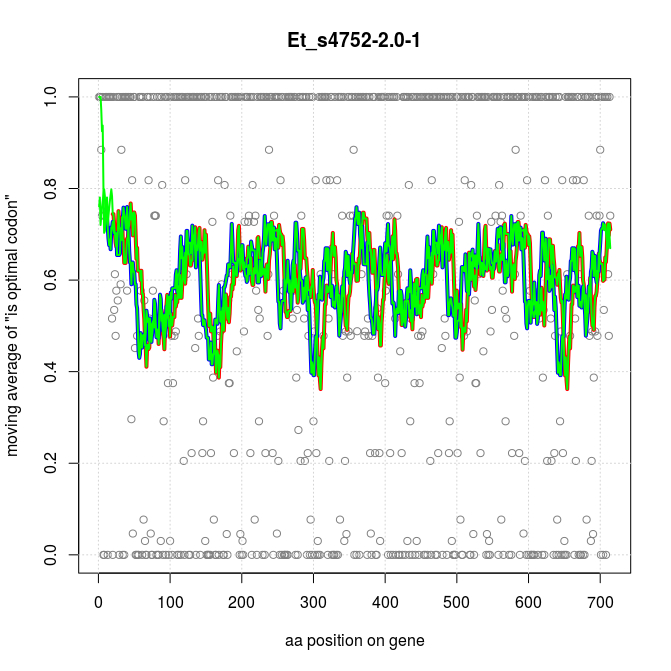
\includegraphics[width=0.5\columnwidth]{fig1_plotOCU} 
\caption[A sample figure from demo plotOCU]{A sample figure (from plot OCU \emph{demo(plot(OCU)}, of statanacoseq, got from \url{https://github.com/fredysiegrist/statanacoseq}).}
\label{fig:plotOCU} 
\end{figure}
